\documentclass[]{article}

\usepackage[utf8]{inputenc}
\usepackage[french]{babel}
\usepackage{color}

\usepackage{amsmath}

\usepackage{url}

\usepackage[left=2.5cm, right=2.5cm, top=2.5cm]{geometry}
\usepackage{multicol, float}

\usepackage[final]{graphicx}
\graphicspath{{./medias/}}

\usepackage{tikz, pgfplots}
\usepackage[all]{xy}
\pgfplotsset{compat=1.5}

\title{Implantation Fonctionnelle \\ d'Algorithmes Géométriques en 3D \\[0.5cm]
  \large Rapport de projet de recherche}
\author{
	Titouan Laurent - Master 1 parcours Image et 3D\\
	Encadrant : Nicolas Magaud
}
\date{}

\begin{document}

\makeatletter
\begin{titlepage}
	\begin{center}
		
\includegraphics[width=0.25\linewidth]{logos/icube.jpg}
		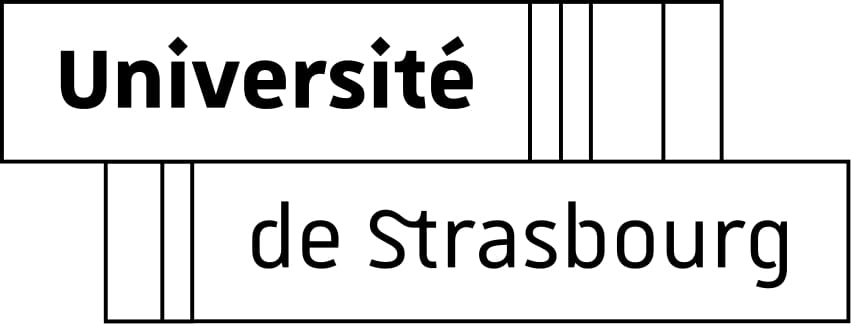
\includegraphics[width=0.3\linewidth]{logos/uds.jpg}\\[2cm]
		{\huge \bfseries  \@title }\\[1cm]
		{\large  \@author}\\[2cm]
		\begin{center}
			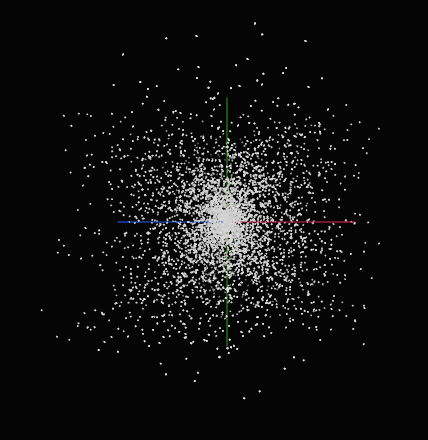
\includegraphics[width=5cm]{illus/illus0.png}
			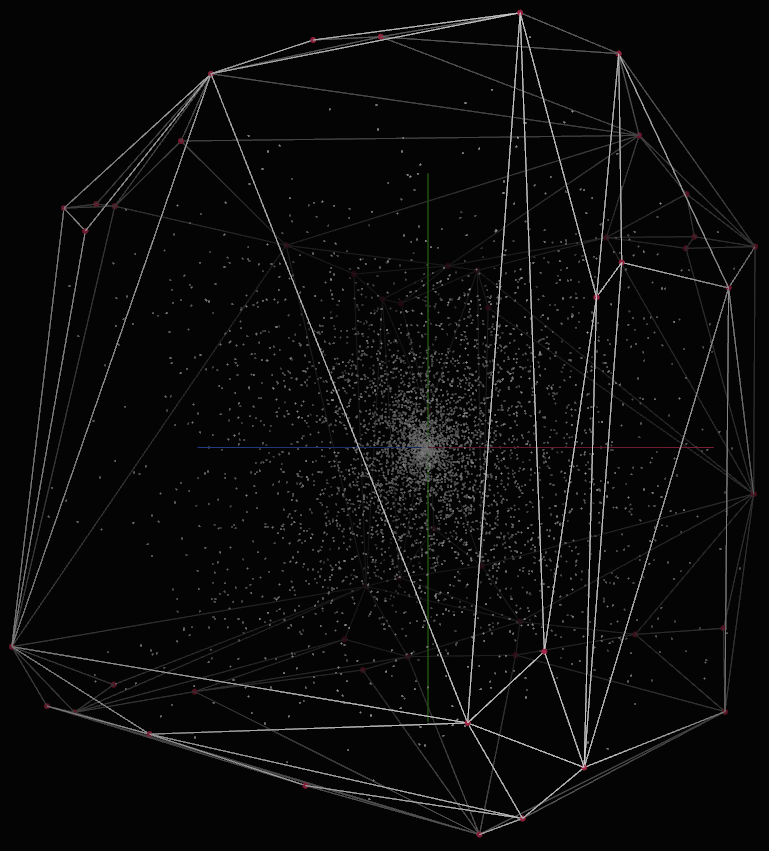
\includegraphics[width=5cm]{illus/illus1.png}
			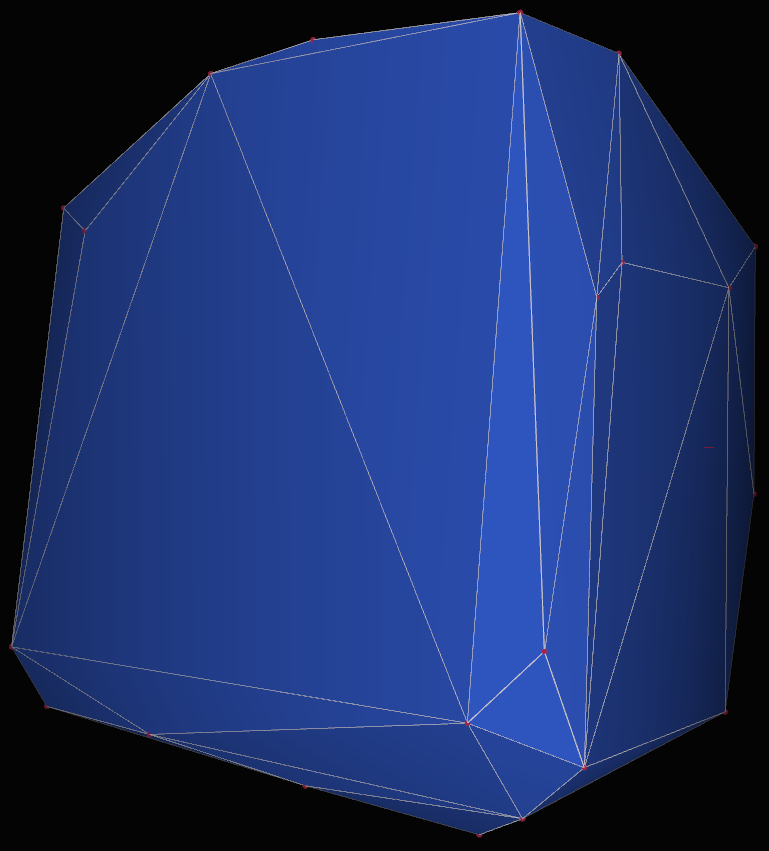
\includegraphics[width=5cm]{illus/illus2.png}
		\end{center}
	\end{center}
\end{titlepage}
\makeatother

\newpage

\newpage
\tableofcontents
\newpage

\section{Introduction}
\paragraph{Preuve assistée par ordinateur}
Prouver la correction d'un algorithme, c'est à dire démontrer formellement qu'il répond à des spécifications précises est une tâche qui se veut essentielle dans de nombreux domaines de l'informatique. Cela permet de s'assurer de sa robustesse et donc de celle des implantations qui en découlent.ggg

Cependant, il peut-être fastidieux de chercher à faire une démonstration formelle à la main, d'autant plus qu'en informatique l'écart entre une implantation donnée et sa description formelle représente une limite. Dans le cas des algorithmes géométriques, il y a l'introduction de difficultés supplémentaires, puisque l'on se retrouvera généralement à travailler aussi bien sur des notions topologiques qu'arithmétiques.

À partir de là, les outils outils de preuve automatique se présentent comme une solution viable. Ils permettent de démontrer des propriétés dans une implantation donnée d'un algorithme, et donc d'en prouver la correction. La contrainte étant que l'implantation doit être faite dans un style de programmation fonctionnel. Leur intérêt réside aussi dans le fait qu'on peut en extraire un programme certifié.

\paragraph{Application au calcul de l'enveloppe convexe}
Le calcul de l'enveloppe convexe d'un ensemble fini de points est un problème bien connu en géométrie et en informatique. Un certain nombre d'algorithmes existent pour le résoudre, et parmi ceux-ci Quickhull se veut être inspiré de Quicksort en proposant une approche de type diviser pour régner, lui assurant une complexité en $O(n\log{}n)$.

Par le passé, une implantation de Quickhull restreinte aux ensembles de points à 2 dimensions a été proposée et prouvée formellement. Seulement, la généralisation de Quickhull aux ensembles à 3 dimensions et plus, à partir de la version précédente, n'est pas une tâche triviale à cause des contraintes supplémentaires de visibilité (qu'on ne retrouve pas en 2 dimensions). Il faut également ajouter que les implantations en 3 dimensions existantes sont le pour la grande majorité faites dans un style de programmation impératif, et donc pas directement adapté à la preuve automatique.

\paragraph{}
Mon travail de recherche a donc pour objectif d'explorer ce qui est envisageable en terme d'implantation en style de programmation fonctionnel, de preuve mais aussi d'aide à la visualisation de l'algorithme Quickhull en 3 dimensions.

\section{Choix d'un langage de programmation}
Pour ce sujet le langage de programmation retenu est celui de Coq. Coq est un assistant à la construction de preuves automatiques, codées avec une syntaxe qui lui est propre, en paradigme fonctionnel.

Seulement, ici il présente au moins quatre limitations importantes :
\begin{itemize}
	\item C'est un langage plutôt austère à prendre en main, sa syntaxe est loin d'être évidente et donc il n'est que peu pratique pour développer rapidement et aisément.
	\item Il ne permet nativement pas de faire du dessin graphique, ce qui serait pourtant très pratique pour vérifier visuellement le bon fonctionnement des programmes développés.
	\item Il en est de même pour la lecture et l'écriture de fichiers (pour stocker l'enveloppe convexe par exemple).
	\item Coq n'est pas un environnement dédié à l'exécution de programmes. En effet il n'est que très peu performant en temps et en capacités de calcul (même lorsqu'il s'agit de faire des opérations arithmétiques sur de simples entiers non signés).
\end{itemize}

\subparagraph{}
J'ai donc porté mon choix sur le \textbf{JavaScript}, et ce pour les raisons suivantes :
\begin{itemize}
	\item Mis à part Coq, je n'ai jamais utilisé de langage purement fonctionnel jusque-là.
	\item Hors, JavaScript, un langage que je connais particulièrement bien, est \textbf{multi-paradigme}, et donc il permet nativement de développer dans un style de \textbf{programmation fonctionnel}.
	\item JavaScript est adapté à la lecture/écriture de fichiers.
	\item JavaScript intègre nativement des outils de \textbf{rendu graphique} (WebGL et dessin dans un Canvas avec des instructions simples).
\end{itemize}

\section{Implantation de Quickhull en 2D en JavaScript}
Avant de commencer à directement travailler sur Quickhull en 3 dimensions, il m'est d'abord bien plus évident de chercher à bien comprendre le cas restreint (et donc plus simple) des ensembles à deux dimensions, ne serait-ce que pour en cerner les caractéristiques principales. Cela passe donc par l'implantation de l'algorithme, qui sera faite dans un style fonctionnel.

\subsection{Principe général}
\paragraph{}
L'algorithme Quickhull en 2 dimensions pourrait être qualifié de "cas d'école" de la technique du \emph{diviser pour régner}. Pour s'en convaincre on peut reprendre l'exemple suivant, illustrant des étapes successives de la construction de l'enveloppe.

\begin{figure}[H]
	\begin{center}
		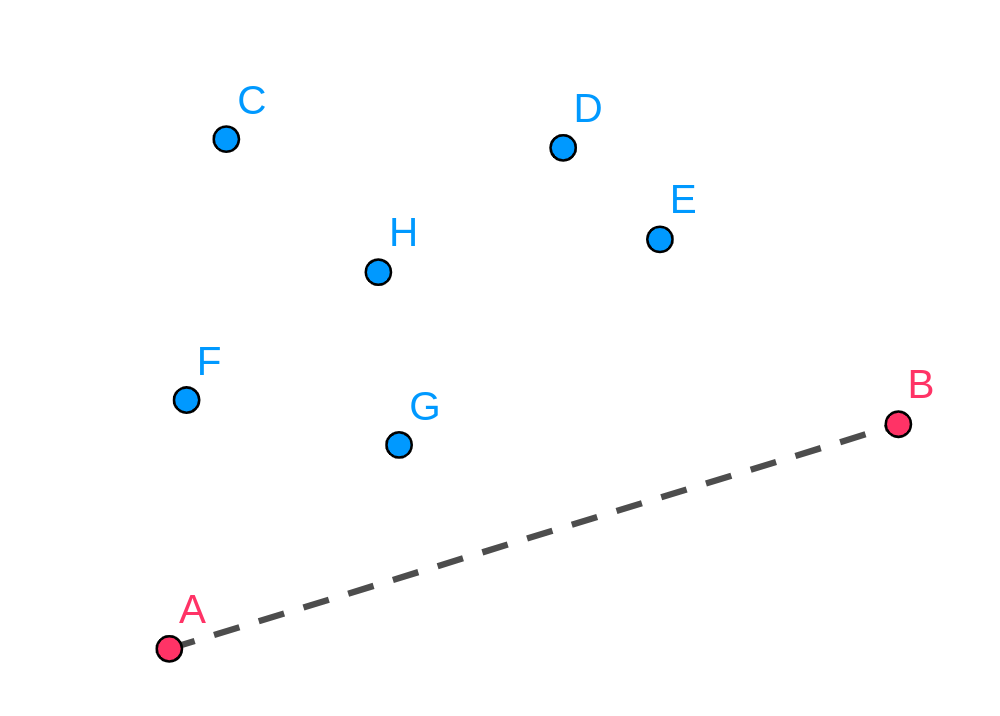
\includegraphics[width=5cm]{qh2d/geogebra-export.png}
		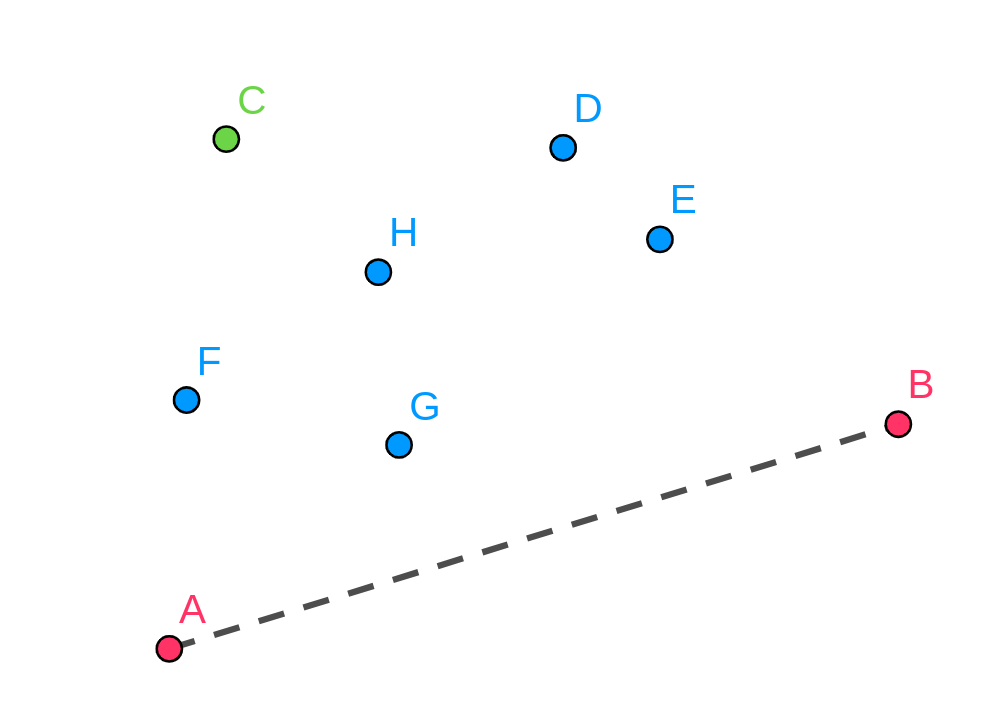
\includegraphics[width=5cm]{qh2d/geogebra-export2.png}
		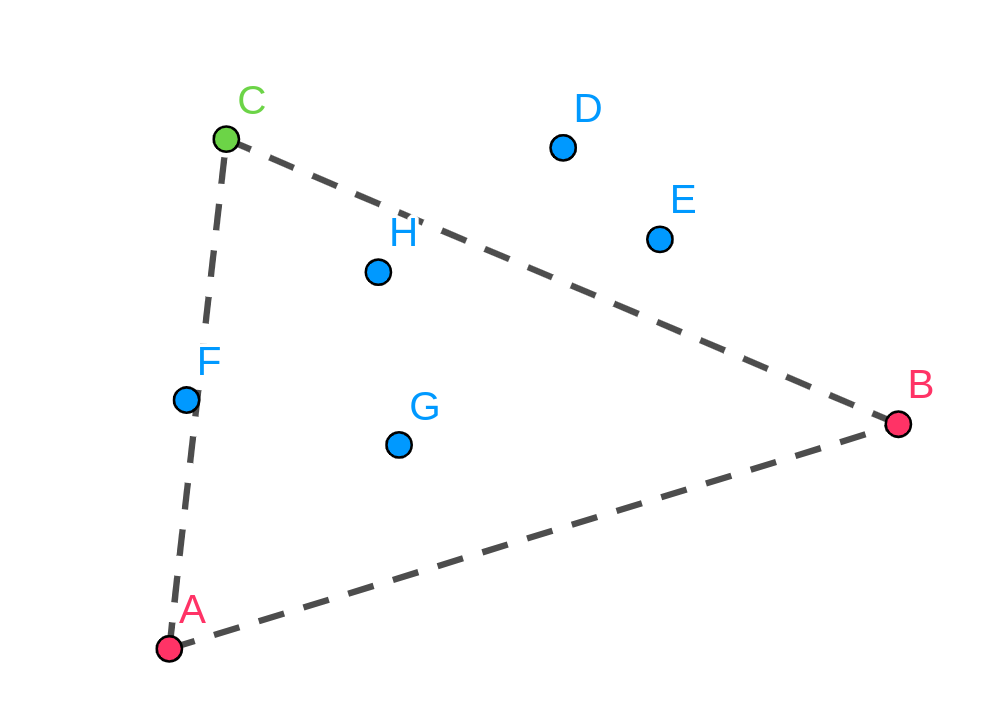
\includegraphics[width=5cm]{qh2d/geogebra-export3.png}
	\end{center}
\end{figure}

Considérons que l'on dispose des points suivants. Supposons également qu'on sait que les points $A$ et $B$ (en rouge) appartiennent à l'enveloppe convexe (arête en pointillé). La prochaine étape de l'algorithme est alors de déterminer le point le plus extrême (le plus éloigné) de l'arête $AB$ : on trouve le point $C$ (en vert).

\begin{figure}[H]
	\begin{center}
		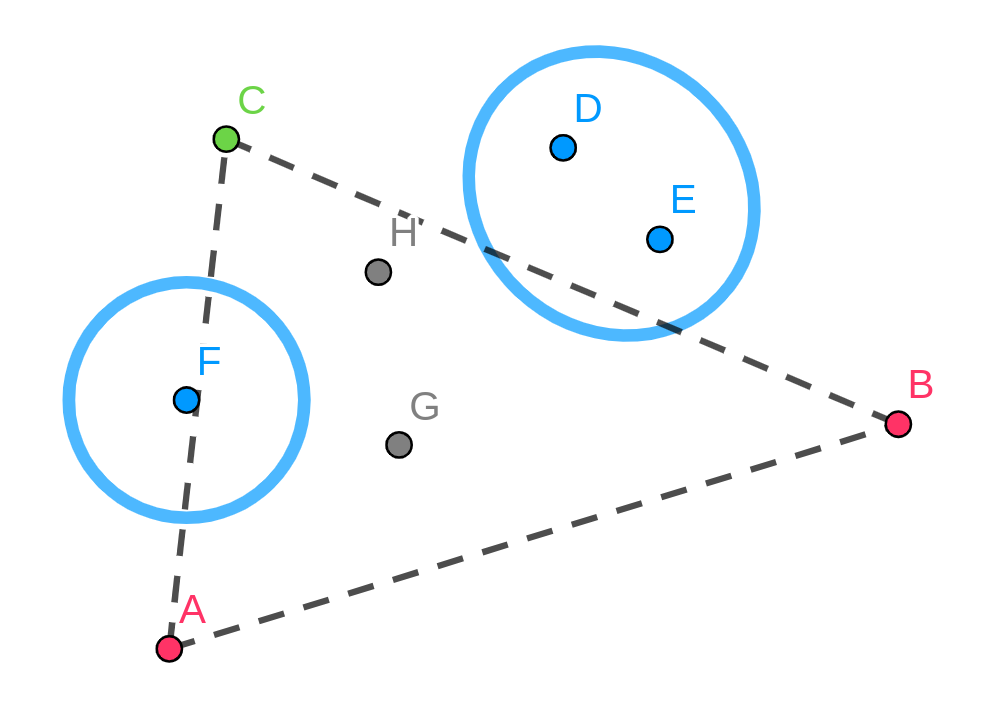
\includegraphics[width=5cm]{qh2d/geogebra-export4.png}
	\end{center}
\end{figure}

Sachant la nouvelle enveloppe obtenue, on peut alors procéder à la division du problème en deux sous-problèmes (plus petits) : pour chaque arête nouvellement créée (ici $AC$ et $CB$), on forme un sous-ensemble de points (entourés en bleu) en ne gardant que ceux qui sont visibles depuis l'arête en question. Ici $H$ et $G$ ne sont pas visibles (visbilité orientée) ni par $AC$, ni par $CB$, donc ils ne font pas partie de l'enveloppe convexe.

On peut alors récursivement appliquer le même algorithme sur les 2 sous-ensembles générés (entourés en bleu ici) par rapport à leur arête respective ($AC$ et $CB$).

L'enveloppe convexe est alors construite par les opérations de combinaison des données de retour des sous-appels récursifs (il s'agit basiquement d'une liste ordonnée des points appartenant à l'enveloppe convexe).

\paragraph{Note :}
Il est important de noter qu'un point fort de cet algorithme réside dans le choix du point le plus extrême par rapport à une arête. Avec cette méthode on s'assure d'avoir deux sous-ensembles disjoints de points associés aux nouvelles arêtes, et donc on peut appliquer le même algorithme sur les 2 sous-ensembles.

Si on n'avait pas l'assurance que les sous-ensembles sont disjoints, on ne pourrait tout simplement pas faire l'opération de division, et donc pas de \emph{diviser pour régner}.

\paragraph{}
La première étape de Quickhull en 2D (et donc des premiers appels récursifs) peut varier en fonction des implantations. Pour ma part j'ai choisi celle qui consiste à prendre les deux points sur un même axe ($x$ ou $y$) qui sont les plus éloignés l'un de l'autre. On obtient une arête dont chacune des extrêmités appartient à l'enveloppe convexe. Il suffit alors de lancer l'algorithme précédent en partant successivement de chacun des (2) côtés de l'arête.

\subsection{Structures de données}
En termes de structures de données il n'y a besoin que de 3 structures principales :
\begin{itemize}
	\item Un point constitué de deux coordonnées flottantes $x$ et $y$.
	\item Une liste (statique) de points dont on va chercher à calculer l'enveloppe convexe.
	\item Une liste (dynamique) d'entiers non signés pour représenter aussi bien les ensembles de points (indices des points) associés à une arête, que ceux formant l'enveloppe convexe (cette liste est ordonnée dans l'ordre de voisinage des sommets des arêtes).
\end{itemize}

Du fait de la simplicité de ces structures, elles ne représentent pas une contrainte particulière pour une implantation en style fonctionnel.

\subsection{Implantation et démo visuelle}
En plus d'implanter Quickhull en 2D en JavaScript, j'ai développé un affichage en WebGL qui permet de visualiser les étapes de l'algorithme sur des exemples. La visualisation est un moyen de vérifier mais aussi de mieux comprendre le fonctionnement de ce qui est implanté.

Les captures qui suivent sont celles dudit affichage, avec le code couleur suivant :
\begin{itemize}
	\item Petits points blancs : ensemble de points dont on souhaite calculer l'enveloppe convexe.
	\item Arête rouge : arête déjà parcourue qui appartient (ou qui a appartenu) à l'enveloppe convexe.
	\item Arête jaune : arête courante sur laquelle la récursion est faite ou arête nouvellement ajoutée à l'enveloppe convexe.
	\item Arête verte : arête appartenant à l'enveloppe convexe finale calculée.
\end{itemize}

\begin{figure}[H]
	\begin{center}
		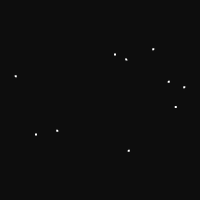
\includegraphics[width=2.5cm]{qh2d/demo2d/frame0.png}
		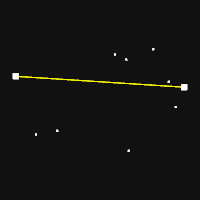
\includegraphics[width=2.5cm]{qh2d/demo2d/frame1.png}
		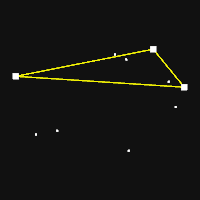
\includegraphics[width=2.5cm]{qh2d/demo2d/frame2.png}
		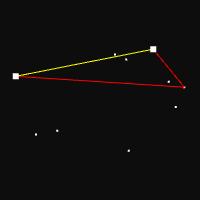
\includegraphics[width=2.5cm]{qh2d/demo2d/frame3.png}
		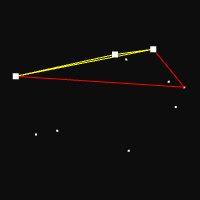
\includegraphics[width=2.5cm]{qh2d/demo2d/frame4.png}
		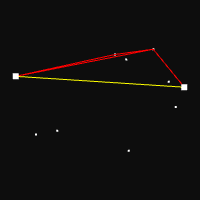
\includegraphics[width=2.5cm]{qh2d/demo2d/frame5.png}
		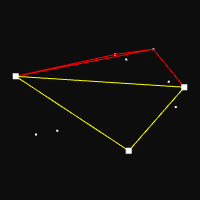
\includegraphics[width=2.5cm]{qh2d/demo2d/frame6.png}
		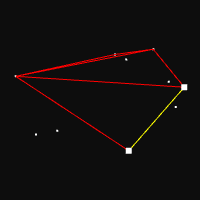
\includegraphics[width=2.5cm]{qh2d/demo2d/frame7.png}
		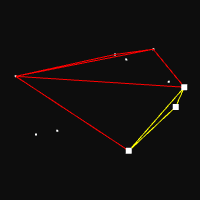
\includegraphics[width=2.5cm]{qh2d/demo2d/frame8.png}
		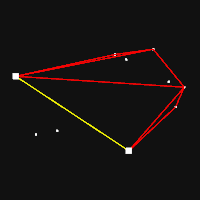
\includegraphics[width=2.5cm]{qh2d/demo2d/frame9.png}
		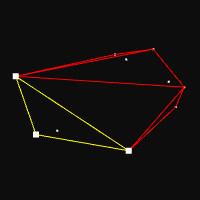
\includegraphics[width=2.5cm]{qh2d/demo2d/frame10.png}
		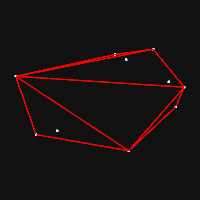
\includegraphics[width=2.5cm]{qh2d/demo2d/frame11.png}
		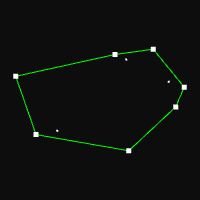
\includegraphics[width=2.5cm]{qh2d/demo2d/frame12.png}
	\end{center}
	\caption{Étapes de construction dans l'ordre chronologique de l'enveloppe convexe 2D sur un exemple simple.}
\end{figure}

\begin{figure}[H]
	\begin{center}
		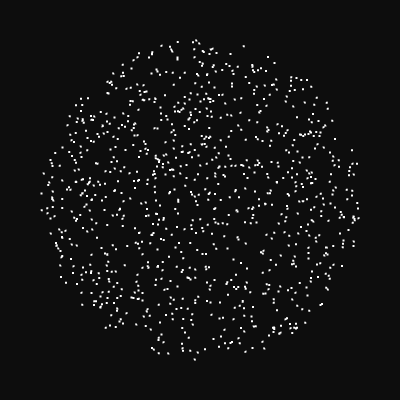
\includegraphics[width=5cm]{qh2d/demo2d/frame_b0.png}
		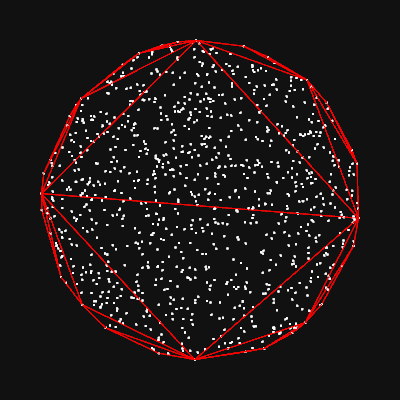
\includegraphics[width=5cm]{qh2d/demo2d/frame_b1.png}
		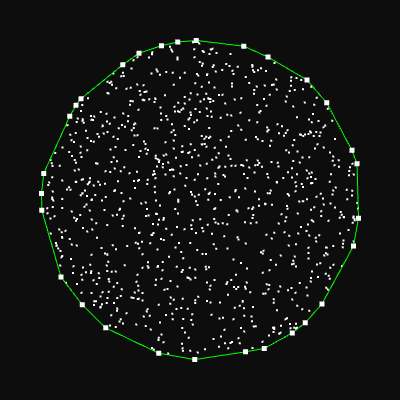
\includegraphics[width=5cm]{qh2d/demo2d/frame_b2.png}
	\end{center}
	\caption{Exemple avec un ensemble de points plus grand, sans toutes les étapes intermédiaires.}
\end{figure}

\section{Implantation de Quickhull en 3D en JavaScript}
Implanter Quickhull restreint aux ensembles de points en 2D s'est révélé être assez simple, malgré la contrainte de devoir programmer en style fonctionnel. Dans cette section on s'attarde sur la version en 3D, qui représente la partie la plus importante de mon travail de recherche.

\subsection{Principe et spécificités}
Au-delà de 2 dimensions, l'algorithme Quickhull est nettement plus complexe à implanter. Déjà, en trois dimensions une enveloppe convexe n'est plus une suite d'arêtes mises bout à bout, mais un maillage surfacique triangulaire. Ce qui va demander de penser à une nouvelle structure de données adaptée.

De plus, il n'est plus possible de faire un algorithme en \emph{diviser pour régner}, et pour le comprendre on va regarder un exemple similaire à celui donné pour Quickhull 2D.

\paragraph{}
\emph{Pour aider à la lisibilité des points dans l'espace 3D, le triangle $ABC$ est sur le plan de la grille, et les points $D$ à $H$ sont représentés avec leur droite verticale.}

\begin{figure}[H]
	\begin{center}
		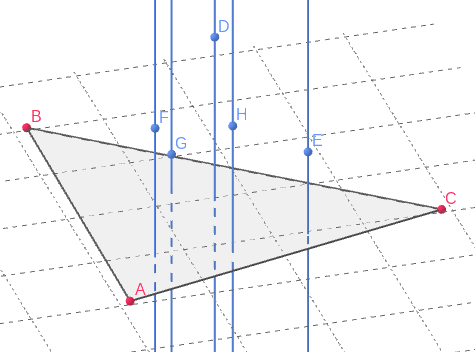
\includegraphics[width=5cm]{qh3d/geogebra-export3.png}
		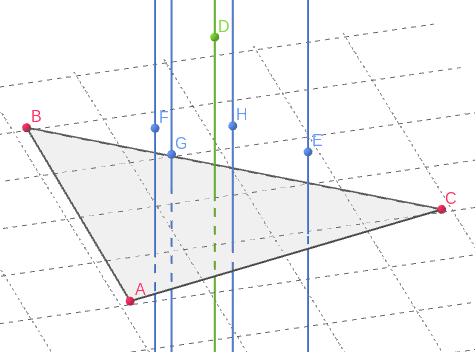
\includegraphics[width=5cm]{qh3d/geogebra-export4.png}
		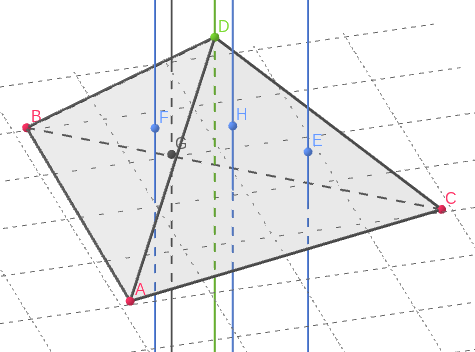
\includegraphics[width=5cm]{qh3d/geogebra-export5.png}
	\end{center}
\end{figure}

Considérons que l'on dispose du triangle $ABC$ : une face de l'enveloppe convexe, et des points $D$ à $H$ comme étant l'ensemble des points non traités. Comme pour Quickhull 2D, on va déterminer le point le plus extrême (le plus éloigné) de la face $ABC$ : on trouve le point $D$ (en vert).

La nouvelle enveloppe est alors obtenue par la construction des trois faces $ABD$, $ACD$, $BCD$. Le prédicat de visibilité nous permet de déterminer que le point $G$ (en gris) n'appartient pas à l'enveloppe convexe car non visible des trois faces.

\paragraph{}
Tout semble bien se passer, jusqu'à l'étape de la division :

\begin{figure}[H]
	\begin{center}
		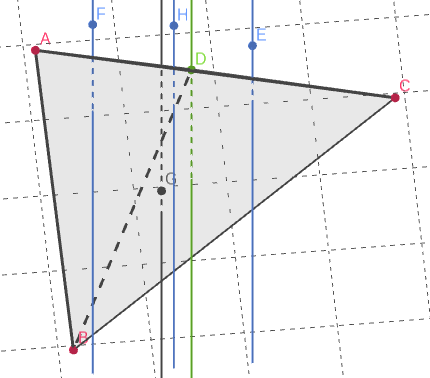
\includegraphics[width=6cm]{qh3d/geogebra-export6.png}
		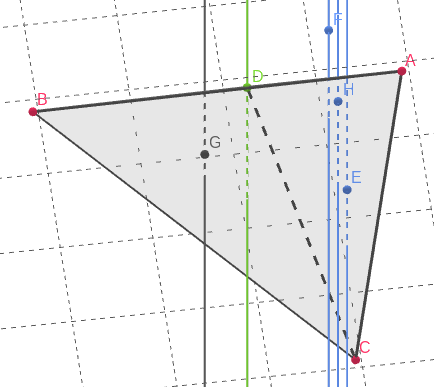
\includegraphics[width=6cm]{qh3d/geogebra-export7.png}
	\end{center}
\end{figure}

Sur ces deux vues on ne fait \textbf{que} de déplacer la caméra autour du solide.
En alignant sur une seule droite successivement les points $A$, $D$ et $C$, puis les points $B$, $D$ et $A$, on peut voir que le point $F$ est visible \textbf{simultanément} par deux des faces nouvellement créées.

Cette particularité nous interdit de faire l'étape de la division pour \emph{diviser pour régner}. On comprend également que contrairement à la version 2D où l'on se contentait de modifier supprimer une arête à la fois pour la subdiviser en de nouvelles sous-arêtes, ici on devra parfois supprimer plusieurs faces (car visibles depuis un point extrême) pour reconstruire un certain nombre de faces supplémentaires (l'exemple donné ici est un cas particulier plutôt simple car le point extrême $D$ ne voit qu'une seule face : le triangle $ABC$).

\subsection{Adaptation de l'algorithme}

Puisque l'on ne peut pas faire de \emph{diviser pour régner}, l'algorithme doit être pensé différemment. Je me suis basé sur le pseudo-code donné dans \cite{10.1145/235815.235821} qui propose une généralisation pour les dimensions supérieures à 2.

\paragraph{}
La boucle principale de l'algorithme suit ces étapes :
\begin{itemize}
	\item On choisit une face parmi les faces de l'enveloppe convexe courante dont le sous-ensembles de points non-traités associé est non-vide.
	\item On prend le point le plus extrême (le plus éloigné) par rapport à ladite face depuis le sous-ensemble de points associé.
	\item On supprime \textbf{toutes} les faces visibles de l'enveloppe convexe depuis ce point.
	\item On reconstruit l'enveloppe convexe en formant des faces (triangles) entre ce point et le bord du trou laissé à l'étape précédente.
	\item On recalcule le sous-ensemble de points associé à la face courante par rapport à la nouvelle enveloppe obtenue (étape qui est loin d'être triviale). On devrait obtenir un nouveau sous-ensemble de points par face nouvellement ajoutée.
	\item Ré-itérer jusqu'à ce qu'il n'y ait plus de sous-ensemble non-vide associé à l'une des faces de l'enveloppe convexe.
\end{itemize}

\paragraph{}
La première étape de l'algorithme consiste (à la manière de Quickhull 2D) à trouver un solide minimal qui formera l'enveloppe convexe initiale. Celui-ci est formé de 4 faces (soient 4 points), sélectionnés suivant la méthode suivante (méthode adaptée de \cite{smith}) :
\begin{itemize}
	\item On cherche deux points les plus éloignés sur deux axes (parmi $x$, $y$ et $z$) parmi l'ensemble de points.
	\item Avec l'arête formée des deux points précédent, on cherche un troisième point le plus éloigné de ce segment.
	\item On dispose maintenant d'une face (un triangle) depuis laquelle on va chercher un quatrième point qui en est le plus éloigné.
	\item On peut dès lors construire le tétrahèdre formé par ces 4 points.
	\item On attribue (arbitrairement) à chaque face un sous-ensemble de points qui lui sont visibles.
\end{itemize}

\paragraph{}
On se rend compte que cette fois-ci il va nous falloir une structure de données pour représenter les sous-ensembles de points associés aux faces. Celle-ci sera appelée $oset$ pour \emph{outside set} par la suite (et $osubset$ pour \emph{outside subset}).

\subsection{Structures de données}
\subsubsection{Données d'entrées}
Un $vec3$ permet de modéliser aussi bien un point qu'un vecteur dans l'espace 3D. Les composantes sont données dans l'ordre usuel $x$, $y$ et $z$ (avec $x, y, z \in \mathbf{R}$).\\
Dans notre implantation, on considèrera une simple liste ordonnée des $n$ points (représentée par la variable globale $GLOBAL\_V\_LIST$) comme étant les données d'entrée du problème à résoudre.

\subsubsection{Stockage et manipulation de l'enveloppe convexe en mémoire}
La structure en liste de demi-arêtes orientées (doubly connected edge list, abrégé DCEL) est parmi les plus communes qu'il soit dès lors que l'on souhaite modéliser un maillage topologique.\\
Ici on implante une version restreinte de cette dernière, puisqu'elle permet de créer maillages triangulaires uniquement — ce qui correspond à notre besoin.

\paragraph{Demi-arête}
Une $he$ (abrévation de halfedge, ou demi-arête) est une structure de données disposant d'informations sur elle-même et son voisinage topologique. Celles-ci sont les suivantes :
\begin{itemize}
	\item $index \in \mathbf{Z}$, un identifiant unique pour la demi-arête, avec :
	      \[
		      \left\{
		      \begin{array}{ll}
			      index = -1   & \mbox{est une demi-arête nulle} \\
			      index \geq 0 & \mbox{sinon}
		      \end{array}
		      \right.
	      \]
	\item $opposite \in \mathbf{Z}$, l'identifiant de la demi-arête opposée, avec :
	      \[
		      \left\{
		      \begin{array}{ll}
			      opposite = -1   & \text{est une demi-arête du bord} \\
			      opposite \geq 0 & \text{sinon}
		      \end{array}
		      \right.
	      \]
	\item $vertex \in \mathbf{N}$, l'indice du sommet incident dont elle est issue.
\end{itemize}

\paragraph{Maillage triangulaire}
Une $dcel$ permet la modélisation d'un maillage topologique triangulaire. Elle dispose des attributs suivants :
\begin{itemize}
	\item $he\_list$, une liste de $he$.
	\item $available\_he\_index \in \mathbf{N}$, le prochain indice non attribué à une $he$ de la liste.
\end{itemize}

\paragraph{Exemple simple en 2D} :

\begin{figure}[H]
	\[\begin{aligned}[c]
			\entrymodifiers={+[o][F]}
			\renewcommand{\labelstyle}{\textstyle}
			\xymatrix@=4em @L=.25ex{
			{}
			\ar @^{-} [d]
			\ar @^{-} [dr]
			 & {}
			\ar @^{-} [l]
			\\ {}
			\ar @^{-} [r]
			 & {}
			\ar @^{-} [u]
			}
		\end{aligned}\rightarrow\begin{aligned}[c]
			\xymatrix@=4em @L=.25ex{
			{\color{red}0}
			\ar @<.25ex> @^{->} [d] |{\color{blue}0}
			\ar @<.25ex> @^{->} [dr] ^{\color{blue}4}
			 & {\color{red}1}
			\ar @<.25ex> @^{->} [l] |{\color{blue}3}
			\\ {\color{red}2}
			\ar @<.25ex> @^{->} [r] |{\color{blue}1}
			 & {\color{red}3}
			\ar @<.25ex> @^{->} [ul] ^{\color{blue}2}
			\ar @<.25ex> @^{->} [u] |{\color{blue}5}
			}
		\end{aligned}\]
	\caption{Un maillage simple et un indiçage correspondant.}
	\label{maillage_simple}
\end{figure}

\begin{figure}[H]
	\[
		\begin{aligned}[c]
			\begin{array}{l}
				\begin{tabular}{|c|c|c|c|}
					\hline
					index         & opposite      & vertex       \\
					\hline
					\color{blue}0 & -1            & \color{red}0 \\
					\hline
					\color{blue}1 & -1            & \color{red}2 \\
					\hline
					\color{blue}2 & \color{blue}4 & \color{red}3 \\
					\hline
					\color{blue}3 & -1            & \color{red}1 \\
					\hline
					\color{blue}4 & \color{blue}2 & \color{red}0 \\
					\hline
					\color{blue}5 & -1            & \color{red}3 \\
					\hline
				\end{tabular} \\\\
				available\_he\_index\textbf{ : }6
			\end{array}
		\end{aligned}
		\begin{aligned}[c]
			\begin{tabular}{|c|c|}
				\hline
				Indice       & Coordonnées \\
				\hline
				\color{red}0 & (0,0)       \\
				\hline
				\color{red}1 & (1,0)       \\
				\hline
				\color{red}2 & (1,1)       \\
				\hline
				\color{red}3 & (0,1)       \\
				\hline
			\end{tabular}
		\end{aligned}
	\]
	\caption{Structure $dcel$ à gauche et la table des sommets à droite.\\\textbf{Note :} $avaiable\_he\_index$ est l'indice pour la prochaine demi-arête qui sera ajoutée à la $dcel$. On pourrait s'en passer et utiliser à la place l'indice de la dernière $he$ ajoutée à la $dcel$ pour calculer le prochain indice.}
	\label{maillage_simple_struct_associee}
\end{figure}

Considérons le maillage de la Figure~\ref{maillage_simple}. Une structure $dcel$ associée valide serait alors telle que celle présentée Figure~\ref{maillage_simple_struct_associee}.

\paragraph*{Note :} si les numéros d'indices choisis pour les demi-arêtes sont ici plus ou moins arbitraires, la structure $dcel$ impose tout de même des contraintes comme nous allons le voir.

\paragraph{Ajout et retrait d'une face dans une $dcel$}
Il s'agit des deux seules opérations de modification d'une $dcel$.

\subsubsection{Stockage et manipulation de l'ensemble de points extérieurs associés aux faces}
\paragraph*{Sous-ensemble de points extérieurs — $osubset$}
Un sous-ensemble de points extérieurs (outside subset) est une structure de données à deux champs :
\begin{itemize}
	\item $face\_index \in \mathbf{N}$, l'identifiant unique d'une face.
	\item $list \in \mathbf{N}$, l'ensemble des points extérieurs à la face $face\_index$, représentés par leur indice dans $GLOBAL\_V\_LIST$.
\end{itemize}

\paragraph*{Ensemble de points extérieurs — $oset$}
L'ensemble de points extérieurs (outside set) n'est rien d'autre qu'une liste d'$osubset$, chacune associée à une unique face (et son ensemble de points extérieurs associé).

\subsection{Évaluation des performances}
Lors d'une itération dans l'algorithme de calcul d'enveloppe convexe 3D, deux instructions successives amènent à devoir choisir un élément parmi un ensemble — sachant que tous conduisent à la terminaison du programme et à la construction d'une enveloppe convexe valide. Dès lors l'utilisation d'heuristiques est envisageable, et cette partie porte sur la comparaison des performances en temps de calcul en fonction des méthodes employées.

Dans la prochaine section on s'intéresse à la sélection du prochain sous-ensemble de points non-vide (et donc implicitement d'une face du polygone convexe en cours de construction).
Tandis qu'à la section suivante on s'intéresse à la sélection du point parmi ceux du sous-ensemble choisit précédemment.

Les tests ont été conduits en moyennant le temps de calcul pour 50 échantillons de points générés aléatoirement (répartition spatiale aléatoire et uniforme).

\paragraph{Heuristique sur le choix du point} :
\begin{figure}[H]
	\begin{center}
		\begin{tikzpicture}
			\begin{axis}[
					title = {},
					xlabel = {Nombre de points en entrée},
					ylabel = {Temps de calcul (ms)},
					legend entries={Point le plus éloigné,Premier point de la liste},
					legend style={at={(0,1)},anchor=north west}
				]
				\addplot+[blue] table {medias/normal.dat};
				\addplot table {medias/not_extreme_point.dat};
			\end{axis}
		\end{tikzpicture}
	\end{center}
	\caption{La courbe bleue montre ici que la stratégie consistant à prendre le point le plus éloigné du plan courant offre de meilleures performances en temps que celle où l'on prend naïvement le premier point de la liste (courbe rouge).}
\end{figure}

\paragraph{Heuristique sur le choix du sous-ensemble} :
\begin{figure}[H]
	\begin{center}
		\begin{tikzpicture}
			\begin{axis}[
					title = {},
					xlabel = {Nombre de points en entrée},
					ylabel = {Temps de calcul (ms)},
					legend entries={Premier sous-ensemble,Plus petit sous-ensemble,Plus grand sous-ensemble},
					legend style={at={(0,1)},anchor=north west},
				]
				\addplot+[blue] table {medias/normal.dat};
				\addplot table {medias/smallest_osubset.dat};
				\addplot table {medias/largest_osubset.dat};
			\end{axis}
		\end{tikzpicture}
	\end{center}
	\caption{
		De manière prévisible choisir le plus petit sous-ensemble à chaque itération nuit aux performances de l'algorithme (courbe rouge). En effet en ne prenant à chaque fois que un plus petit sous-ensemble de $n$ points (avec $n > 0$), on se restreint alors à retirer de l'ensemble total $n$ points au mieux à cette itération.\\
		Il est intéressant de noter ici que prendre le plus grand sous-ensemble (courbe brune) est plus performant que de choisir le premier de la liste (courbe bleue), mais le gain n'est pas aussi significatif que ce qu'on a montré précédemment.
	}
\end{figure}

\subsection{Démo visuelle}
De la même manière que pour la version 2D, j'ai développé un affichage de l'algorithme de calcul d'enveloppe convexe 3D avec WebGL. Celui-ci s'est avéré absolument indispensable pour débugger le code tout au long du développement. Au final il permet également de visualiser, étape par étape, la construction des différentes faces de l'enveloppe convexe.

\begin{figure}[H]
	\begin{center}
		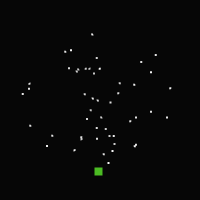
\includegraphics[width=2.65cm]{qh3d/demo3d/init_6.png}
		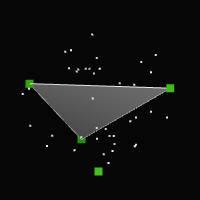
\includegraphics[width=2.65cm]{qh3d/demo3d/init_5.png}
		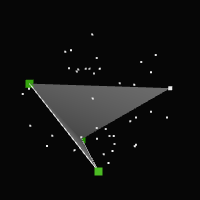
\includegraphics[width=2.65cm]{qh3d/demo3d/init_4.png}
		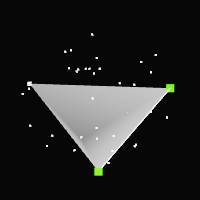
\includegraphics[width=2.65cm]{qh3d/demo3d/init_3.png}
		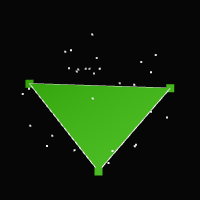
\includegraphics[width=2.65cm]{qh3d/demo3d/init_2.png}
		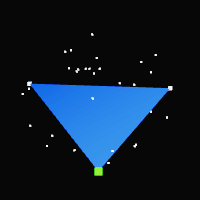
\includegraphics[width=2.65cm]{qh3d/demo3d/init_1.png}
	\end{center}
	\caption{Exemple d'étapes, dans l'ordre chronologique, de la construction de l'enveloppe initiale (tétrahèdre) sur un ensemble de points 3D, face après face.}
\end{figure}

\begin{figure}[H]
	\begin{center}
		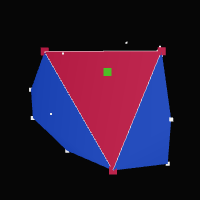
\includegraphics[width=2.65cm]{qh3d/demo3d/add_rem_10.png}
		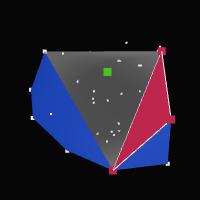
\includegraphics[width=2.65cm]{qh3d/demo3d/add_rem_9.png}
		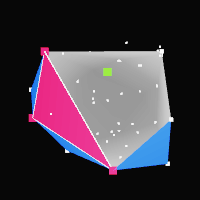
\includegraphics[width=2.65cm]{qh3d/demo3d/add_rem_8.png}
		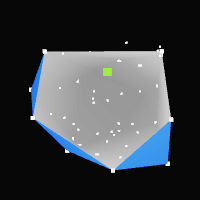
\includegraphics[width=2.65cm]{qh3d/demo3d/add_rem_7.png}
		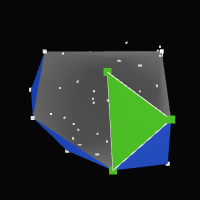
\includegraphics[width=2.65cm]{qh3d/demo3d/add_rem_6.png}
		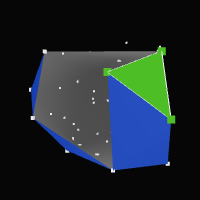
\includegraphics[width=2.65cm]{qh3d/demo3d/add_rem_5.png}
		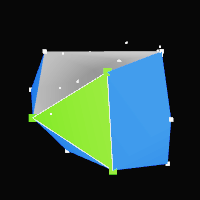
\includegraphics[width=2.65cm]{qh3d/demo3d/add_rem_4.png}
		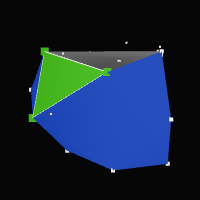
\includegraphics[width=2.65cm]{qh3d/demo3d/add_rem_3.png}
		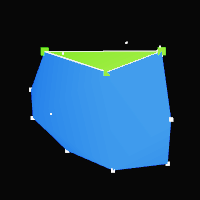
\includegraphics[width=2.65cm]{qh3d/demo3d/add_rem_2.png}
		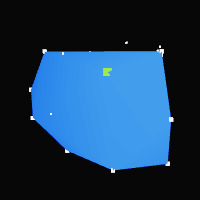
\includegraphics[width=2.65cm]{qh3d/demo3d/add_rem_1.png}
	\end{center}
	\caption{Exemple d'étapes, dans l'ordre chronologique, de la suppression (en rouge) des faces visibles depuis un point extrême sélectionné (en vert), puis de la reconstructions de nouvelles faces (en vert) depuis le contour du trou engendré, avec ledit point.}
\end{figure}

\begin{figure}[H]
	\begin{center}
		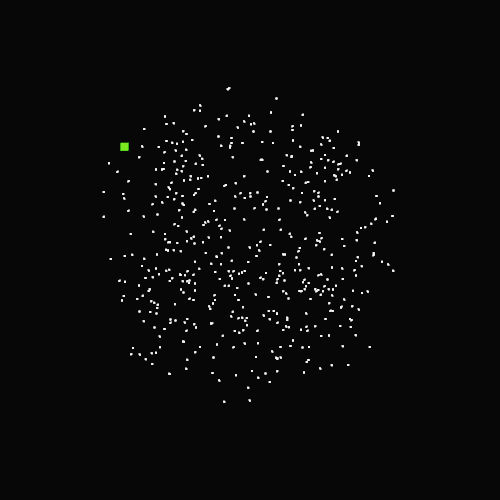
\includegraphics[width=4cm]{qh3d/demo3d/main_0.png}
		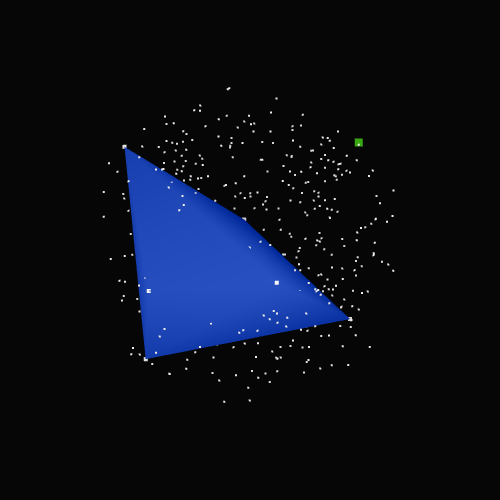
\includegraphics[width=4cm]{qh3d/demo3d/main_1.png}
		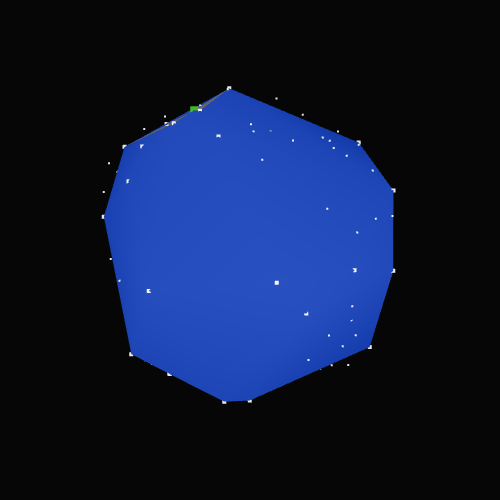
\includegraphics[width=4cm]{qh3d/demo3d/main_2.png}
		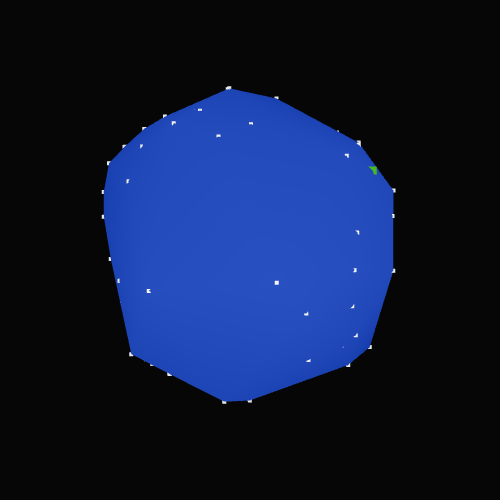
\includegraphics[width=4cm]{qh3d/demo3d/main_3.png}
	\end{center}
	\caption{Dernier exemple sur un grand ensemble de points, engendrant un nombre de faces élevé.}
\end{figure}

\section{Implantation d'une étape de Quickhull 3D en Coq et extraction en Haskell}
Maintenant que nous avons une implantation de Quickhull 3D qui fonctionne dans un style de programmation fonctionnelle, il serait intéressant d'explorer ce qu'il est possible de faire avec Coq. Pour rappel, l'idée à terme serait d'utiliser Coq pour prouver formellement que notre implantation de Quickhull 3D est correcte.

\subsection{Variations par rapport à l'implantation JavaScript}
Pour cette ré-implantation en Coq, je n'ai pas ré-écrit tout l'algorithme de Quickhull 3D, ni toutes ses structures de données. Le temps qu'il me restait m'aurait été bien insuffisant pour cela. L'idée c'est plutôt d'avoir une preuve de concept, et donc j'ai décidé de n'implémenter que la première partie de l'algorithme qui consiste à \textbf{calculer une enveloppe initiale}.

Ainsi ce que j'ai implanté sont les $vec3$ (pour représenter les points en 3 dimensions), des opérations arithmétiques sur ces mêmes $vec3$, des opérations sur les listes, les $he$ et les $dcel$ avec leurs méthodes (à l'exception de l'opération de suppression de face).

\paragraph{Des détails d'implantation ont été revus par rapport à la version en JavaScript}
L'exemple le plus parlant est celui d'avoir utilisé la valeur $-1$ à chaque fois qu'il y a un indice qui peut être non-défini (habitude qui me vient du C). En Coq (et en programmation fonctionnelle de manière générale), on peut faire mieux que cela en utilisant des monades. Les monades apportent une réelle sémantique, qui est explicite (une valeur peut-être non-définie), contrairement au fait de choisir une valeur constante arbitraire, qui elle serait spécifique à l'implantation.

J'ai étendu l'utilisation de monades partout où cela me paraissait pertinent (par exemple, pour les opérations d'accès par indice dans une liste). L'intérêt est aussi d'avoir des garde-fous à plusieurs endroits du programme.

\subsection{Extraction du code Coq}
Dans l'introduction nous avons vu que Coq n'est pas fait pour exporter ou importer des fichiers (autre que des fichiers Coq compilés). Il est aussi très limité en termes de capacités d'exécution de code.

Cependant, l'un de ses modules permet de faire ce que l'on appelle de \textbf{l'extraction de code}. Cette opération consiste à transformer du code source écrit en Coq en un code source écrit dans un autre langage fonctionnel, au choix. Ce que l'on voudrait donc c'est de pouvoir compiler ce code extrait dans un autre langage, pour pouvoir ensuite l'exécuter et se convaincre visuellement de son fonctionnement.

\subsubsection{Choix du langage d'extraction}
Les langages d'extraction supportés par Coq sont au nombre de quatre. À savoir : OCaml, Haskell, Scheme et JSON (qui n'est pas un langage de programmation, mais de stockage de données). Vient alors la question de choisir le langage d'extraction qui sera utilisé.

\subparagraph*{JSON}
Ma première idée fut de choisir JSON plutôt qu'un autre. En effet, je n'ai aucune connaissance de ces autres langages, et j'ai d'abord estimé qu'il serait plus long pour moi de me former à l'un de ceux-ci. De plus, le JSON est extrêmement simple à comprendre et à utiliser, il le serait d'autant plus lorsqu'il s'agira de le raccorder à ce que j'avais déjà développé en JavaScript.

Seulement voilà, comme il ne s'agit que de données, l'agencement à l'intérieur d'un fichier JSON est purement arbitraire. Hors l'extraction de Coq vers ce format n'est absolument pas documenté. Il n'y a même aucune assurance pour que le code extrait soit correct.

Faire la rétro-ingénierie des fichiers extraits depuis Coq aurait été d'une part difficile, mais en plus excessivement long à réaliser, sans aucune garantie de succès.

JSON n'est donc plus un choix viable à ce stade.

\subparagraph*{OCaml, Haskell et Scheme}
Qu'en est-il des autres langages ? Je ne les connais pas, cependant mon choix se portera sur Haskell et ce pour les raisons (subjectives) suivantes :
\begin{itemize}
	\item Sa documentation (Hoogle) me parait être la plus accessible.
	\item Il a une grande communauté de développeurs, donc potentiellement plus de personnes qui rencontrent les mêmes difficultés de débutant que moi.
\end{itemize}

\subsubsection{Extraction de Coq vers Haskell}
L'extraction de code source depuis Coq est une procédure relativement simple mais avec des contraintes assez particulières. De fait, nativement Coq n'implante pas l'extraction de tous les types et structures de données. Le problème se pose alors dans notre cas pour les types de données \texttt{nat} (entiers naturels), \texttt{bool} et \texttt{float}. Des opérations aussi simples, telles que l'addition, la soustraction, le moins unaire de nombres flottants, ou encore la déclaration de constantes flottantes sont tout simplement indéfinies lors de l'extraction.

Une grande partie de mon travail ici aura donc été d'écrire toutes les règles d'extraction indéfinie de Coq vers Haskell. Des exemples donnés page 25 de \cite{magaud:hal-01066671} m'ont bien aidé à comprendre la syntaxe de ces instructions. Ce travail nécessite d'assimiler aussi bien le fonctionnement et la syntaxe de Coq, que celle de Haskell, qui est bien différente.

\subsection{Optimisations et évaluation des performances}

\subsection{Visualisation de la sortie du programme}

\begin{figure}[H]
	\begin{center}
		\includegraphics[width=5cm]{viewer/screen1.png}
	\end{center}
	\caption{Le programme de visualisation fonctionne également avec les enveloppes générées par la version JavaScript de Quickhull 3D.}
\end{figure}

\section{Conclusion}
\subsection{Si c'était à refaire}
\subsection{Pour continuer}

\newpage
\bibliographystyle{plain}
\bibliography{refs}

\end{document}